\documentclass{article}
\usepackage[utf8]{inputenc}
\usepackage{hyperref}
\usepackage{listings}
\usepackage{multimedia} % to embed movies in the PDF file
\usepackage{graphicx}
\usepackage{comment}
\usepackage[english]{babel}
\usepackage{amsmath}
\usepackage{amsfonts}
\usepackage{wrapfig}
\usepackage{multirow}
\usepackage{verbatim}
\usepackage{float}
\usepackage{cancel}
\usepackage{caption}
\usepackage{subcaption}
\usepackage{mathdots}
\usepackage{/home/cade/Homework/latex-defs}


\title{AMATH 575 Problem Set 3}
\author{Cade Ballew \#2120804}
\date{May 10, 2023}

\begin{document}
	
\maketitle
	
\section{Problem 1}
Consider the 2-D map
\begin{equation*}
	\left\{\begin{array}{l}
		x_{n+1} = -x_n + x_n y_n \\
		y_{n+1} = - \frac{y_n}{2} - x_n y_n - x_n^2  
	\end{array}\right..
\end{equation*}
Using Mathematica, we find that the only real fixed point is given by $(x,y)=(0,0)$. Computing the Jacobian at this fixed point,
\[
Df(0,0)=\begin{pmatrix}
-1&0\\
0&-1/2
\end{pmatrix},
\]
is diagonal, so we do not need to transform into eigenspace to get the center manifold and just set $y=h(x)$ and plug this in to get
\[
-h(x)/2-xh(x)-x^2=h(-x+xh(x)).
\]
To find a polynomial expansion for the center manifold up to order 3, we set $h(x)=ax+bx^2+cx^3$. Using Mathematica to collect coefficients, we get the system of equations 
\begin{align*}
a/2=0,\\
-1 - a - a^2 - 3 b/2 = 0,\\
-b + a b + c/2 = 0.
\end{align*}
Solving this with Mathematica, we get
\[
y=-\frac{2x^2}{3}-\frac{4x^3}{3},
\]
as our center manifold. This means that the map restricted to the center manifold is given by
\[
x\to-x-\frac{2x^2}{3}-\frac{4x^3}{3}.
\]
Using Mathematica, we plot this map, from which we can see that the origin is attracting, and thus, the fixed point at the origin is asymptotically stable (Theorem 18.4.2). \\
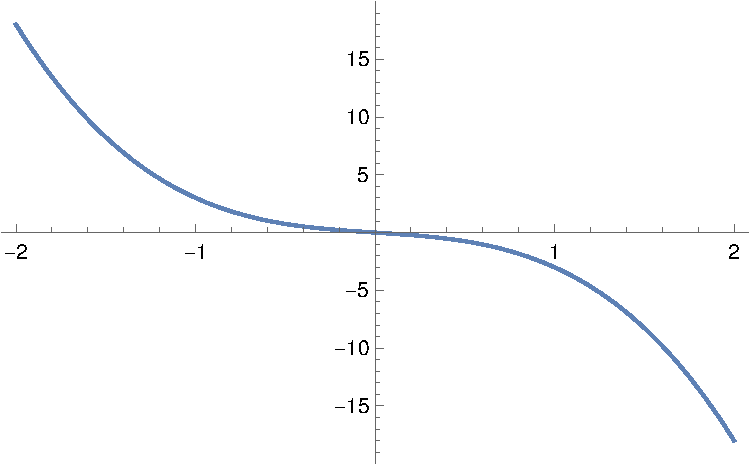
\includegraphics{plot.pdf}

\section{Problem 2}
From Theorem 6.0.1 and Corollary 6.0.2, we can immediately see that in Figure 4.1.2, subfigures b, e, and f cannot occur. This is because periodic orbits must have index $+1$, but the sum of the indices of the fixed points inside this orbit is zero in each case.

\section{Problem 3}
\subsection{Part a}
The fact that gradient vector fields cannot have periodic orbits is a direct result of Theorem 15.0.3. From class, we have that every point of a periodic is an $\omega$ limit point, so Theorem 15.0.3 implies that every point in a periodic orbit is an equilibrium point which is obviously a contradiction. 

\subsection{Part b}
To see that gradient vector fields cannot have homoclinic orbits, we consider such an orbit $\Gamma$ with fixed point $\bar x$. By proposition (15.0.1), $\dot V(\bar x)=0$ and $\dot V(x)\leq0$ for $x\in\Gamma$. Since this curve starts and ends in a neighborhood of $\bar x$, continuity implies that $\dot V(x)=0$ for $x\in\Gamma$. Thus, 
\[
0=\dot V(x)=-|\nabla V(x)|^2,
\]
for $x\in\Gamma$, so $\dot x=0$ for all points on the homoclinic orbit which is a contradiction.

\subsection{Part c}
Finally, to see that gradient vector fields cannot have heteroclinic cycles, we consider such a cycle $\Gamma$ with fixed points $\bar x_1,\ldots \bar x_n$ in that order. Then, the fact that $\dot V(\bar x_j)=0$ for $j=1\ldots,n$ and $\dot V(x)\leq0$ for $x\in\Gamma$ along with continuity implies that 
\[
V(\bar x_1)\geq\ldots\geq V(\bar x_n).
\]
However, the last connection in the cycle implies that 
\[
V(\bar x_n)\geq V(\bar x_1),
\]
so we must have that 
\[
V(\bar x_1)=\ldots=V(\bar x_n),
\]
so $\dot V(x)=0$ for $x\in\Gamma$. Thus, the same argument as in part b implies that $\dot x=0$ for all points on the heteroclinic cycle which is a contradiction.

\section{Problem 4}
Consider the ``all-to-all'' coupled system of phase oscillators on the N-dimensional torus, with coupling strength $\alpha>0$:
\begin{equation*}
	\dot \phi_i = - \alpha/N \sum_{j=1}^N f(\phi_j - \phi_i) \, \, \,  mod \; \; 2 \pi  
\end{equation*}
$i=1...N$ where $f$ is an odd function. To see that this is a gradient system, consider 
\[
V= \frac{\alpha}{N}\sum_{i=1}^{N-1} \sum_{j=i+1}^{N} G(\phi_j - \phi_i),
\]
where $G$ is an anti-derivative of $f$. Then,
\begin{align*}
\left(\nabla V\right)_k=\frac{\alpha}{N}\left(\sum_{j=k+1}^Nf(\phi_j-\phi_k)+\sum_{i=1}^{k-1}f(\phi_k-\phi_i)\right)=\frac{\alpha}{N}\sum_{j=1}^N f(\phi_j - \phi_k).
\end{align*}
Thus, this is indeed a gradient system.

\section{Problem 5}
Consider the 2-D flow
\begin{equation*}
	\left\{\begin{array}{l}
		\dot x = y \\
		\dot y = \mu_1 x - x^3 + \mu_2 y - x^2 y  
	\end{array}\right..
\end{equation*}
We use Bendixson's criterion to show that this system has no periodic orbits for any $\mu_1 \in \mathbb{R}$ and $\mu_2 < 0$. To do this, we compute
\[
\pp{f}{x}+\pp{g}{y}=\mu_2-x^2<0,
\]
for all $x,y\in\real$. Thus, taking $D=\real^2$, Bendixson's criterion implies that there are no closed orbits in $\real^2$.

\section{Problem 6}
Consider the Lorenz equations
\begin{align*}
&\dot x=\sigma(y-x),\\
&\dot y=\rho -y-xz,\\
&\dot z=-\beta z+xy.
\end{align*}
We compute the divergence
\[
\nabla\cdot f=-\sigma-1-\beta,
\]
which is constant. Then, we can use (7.6.3) in Wiggins to get that the volume evolves according to
\[
V(t)=\ex^{-(\sigma+1+\beta)t}V(0),
\]
which is strictly decreasing.

\section{Problem 7}
The divergence free property of a vector field does not necessarily imply that the vector field has a first integral. While one may be tempted to take it to be $I(t)=V(t)$, $V(t)$ is constant while integrals must be nonconstant. As an example of nonexistence, consider the vector field 
\[
\dot x=c,
\]
where $c\in\real$. Then, it must hold that 
\[
\dot I(x)=\nabla I(x)f(x)=c\nabla I(x)=0,
\]
implying that $I$ must be constant and therefore not an integral.

\end{document}
